\documentclass[12pt,a4paper]{article}
\usepackage[utf8]{vietnam}
\usepackage{amsmath,amssymb}
\usepackage{tikz,pgfplots,tkz-tab}
\usepackage{tcolorbox}
\usepackage{multicol,longtable,booktabs,multirow}
\usepackage[version=4]{mhchem}
\usepackage{siunitx}
\usetikzlibrary{calc,patterns,arrows.meta,decorations.pathmorphing}
\pgfplotsset{compat=1.18}
\newcommand{\bonpa}[4]{\par\noindent\textbf{A.} #1 \quad \textbf{B.} #2 \quad \textbf{C.} #3 \quad \textbf{D.} #4\par}
\newcommand{\dinhnghia}[1]{\textbf{Định nghĩa.} #1}
\begin{document}

\section*{Bộ kiểm thử cấu trúc lạ}

\textbf{Câu 1.} Công thức quen: $\displaystyle\int_0^1 \frac{x^2}{\sqrt{1+x^3}}\,dx$ và $\ce{2H2 + O2 -> 2H2O}$, đo $9.8\,\mathrm{m}/\mathrm{s}^2$.
\par\noindent\textbf{A.} $1$.   \textbf{B.} $2$.   \textbf{C.} $3$.   \textbf{D.} $4$.\par

\textbf{Câu 2.} Bảng biến thiên tkz-tab:
\begin{center}
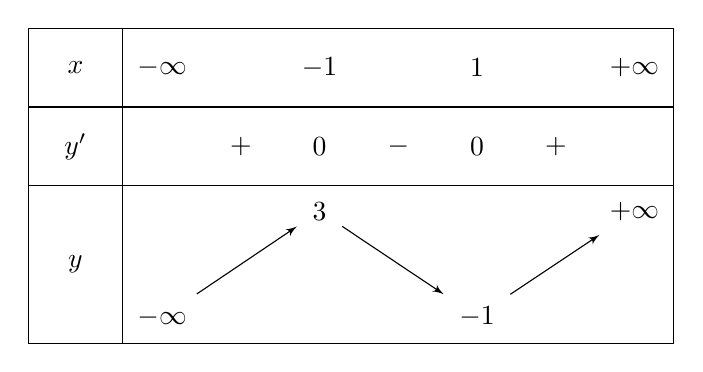
\begin{tikzpicture}
\tkzTabInit[lgt=1.2,espcl=2]{$x$/1,$y'$/1,$y$/2}{$-\infty$,$-1$,$1$,$+\infty$}
\tkzTabLine{,+,0,-,0,+,}
\tkzTabVar{-/$-\infty$,+/$3$,-/$-1$,+/$+\infty$}
\end{tikzpicture}
\end{center}

\textbf{Câu 3.} Đồ thị pgfplots:
\begin{center}


ZLZIMGZ00001ZEND


\end{center}

\textbf{Câu 4.} Khung tcolorbox bo góc có bóng:


\textbf{Ghi nhớ quan trọng}


Với mọi $a,b>0$ ta có $\dfrac{a+b}{2}\ge\sqrt{ab}$.




\textbf{Câu 5.} Hình TikZ vẽ tay có hoa văn và mũi tên lạ:
\begin{center}


ZLZIMGZ00002ZEND


\end{center}

\textbf{Câu 6.} Môi trường HOÀN TOÀN LẠ chưa ai khai báo:



 $x$ $-\infty$ $0$ $+\infty$ 
 $f'$ $+$ $0$ $-$ 




\textbf{Câu 7.} Lệnh lạ chưa ai khai báo:  parabol y=x^2  và  xanh .

\textbf{Câu 8.} Gói chắc chắn KHÔNG có trên máy:
\begin{center}



 1 2 



\end{center}

\textbf{Câu 9.} Bảng dài nhiều cột:
\begin{center}
\begin{tabular}{|c|c|c|c|}
\hline
\multirow{2}{*}{Nhóm} & \multicolumn{3}{c|}{Tần số} \\ \cline{2-4}
 & $n_1$ & $n_2$ & $n_3$ \\ \hline
$[0;5)$ & 3 & 5 & 7 \\ \hline
\end{tabular}
\end{center}

\textbf{Định nghĩa.} Hàm số liên tục trên đoạn $[a;b]$ nếu \ldots

\end{document}
